\documentclass[a4paper,12pt]{article}

\usepackage{préambule}
\usepackage{préambule-figures}
\usetikzlibrary{calc,positioning}

\title{Patron d'un cylindre}
\author{}
\date{}

\begin{document}

\maketitle

\begin{center}
	\begin{tikzpicture}[scale=2]
		\cylindre{3}{2}{0.5};
		\draw[blue,<->] (0,0.5) -- node[midway,above] {\color{blue}2cm} ++(1,0);
		\draw[red,<->] (-1.3,0) -- node[midway,left] {\color{red}5cm} ++(0,-3);
	\end{tikzpicture}
\end{center}

\uline{Consignes} :
\begin{itemize}
	\item Calcule le périmètre de la base de ce cylindre.
	\item Sur une feuille blanche, dessine le patron de ce cylindre, \textbf{en respectant les dimensions !}

	      \begin{center}
		      \begin{tikzpicture}
			      \cylindre{3}{2}{0.5};

			      \draw[\myArrow] (1.6,-1.5) -- ++(0.8,0);

			      % Top and bottom
			      \draw[rotate around={20:(3,0)}] (4,0) ellipse (1 and 0.25);
			      \draw[rotate around={-20:(3,-3)}] (4,-3) [partial ellipse=70:-180:1 and 0.25];

			      \draw (4,0) [partial ellipse=63:0:1 and 0.3] -- ++(0,-3);
			      \draw (4,-3) [partial ellipse=70:0:1 and 0.3];
			      \draw (4,0) [partial ellipse=-180:-70:1 and 0.5] -- ++(0,-3);
			      \draw (4,-3) [partial ellipse=-70:-180:1 and 0.5];
			      \draw (3,0) -- ++(0,-3);

			      \draw[\myArrow] (5.6,-1.5) -- ++(0.8,0);

			      \node at (8,-1.5) {{\Huge ?}};
		      \end{tikzpicture}
	      \end{center}
\end{itemize}

\begin{greybox}[frametitle={Rappel}]
	\begin{minipage}{0.75\textwidth}
		La formule du périmètre d'un cercle de rayon $r$ est
		$$ 2 × r × π $$
	\end{minipage}
	\begin{minipage}{0.25\textwidth}
		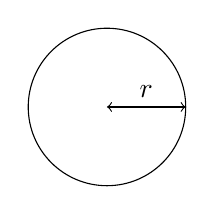
\begin{tikzpicture}
			\draw (0,0) circle (1);
			\draw[<->] (0,0) -- node[midway,above] {$r$} ++(1,0);
		\end{tikzpicture}
	\end{minipage}
\end{greybox}

\end{document}